\section{Tutorials 4 (21 III 2019)}
A game $G = \langle B, W \rangle$\\
$B = \langle V, E, \lambda, v_I \rangle$\\
$E \subseteq V$, $\lambda\ :\ \rightarrow \Gamma$, $v_I \in V$\\
$W \subseteq \Gamma^{*} \cup \Gamma^{\omega}$\\
$\Phi\ :\ \Gamma^{\omega} \rightarrow [0, 1]$\\
$\Phi_W(x) = \begin{cases}
1,\ x \in W\\
0,\ x \not\in W
\end{cases}$\\

\noindent
Example:
\begin{figure}[H]
	\centering
	\caption{Consider this simple game on graph}
	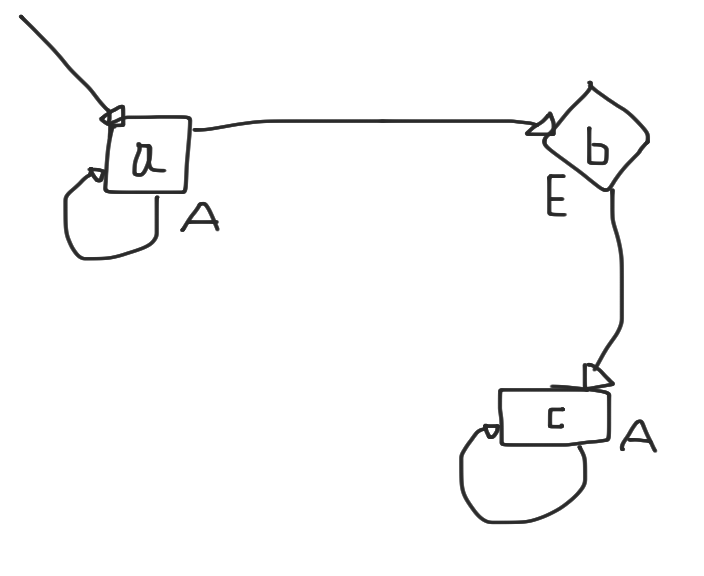
\includegraphics[scale=0.2]{content/graphics/game1.png}
\end{figure}
\noindent
$W = \{w \in \{a, b, c\}^{\omega}\ |\ \exists_{n < \omega} w = a^nb^nc^{\omega}\}$ -- Adam has a winning strategy
(he can infinitely loop in \texttt{a}).\\

\noindent
Strategies for Eve and Adam:\\
$E:\ \delta\ :\ V^{*}V_E \rightarrow V$ s.t. $\delta(w, v) \rightarrow (v')$ (and $v,v' \in E$)\\
$A:\ \pi\ :\ V^{*}V_A \rightarrow V$\\
Or positional strategies:
$\delta\ :\ V_E \rightarrow V$\\
$\pi\ :\ V_A \rightarrow V$\\
A play:\\
$G<\delta, \pi> \rightarrow v_0v_1v_2...v_n.... = p$\\
$w = \lambda(v_0)\lambda(v_1)...\lambda(v_n)...$\\
$w \in W \Leftrightarrow \delta\text{ wins with }\pi$\\

\noindent
(still considering the game above)\\
$W_2 = W \cup \{a^{\omega}\}$ -- Eve has a winning strategy (but not a positional one)\\

\noindent
Reachability game (same graph as before):\\
$W = \Gamma^{*}c\Gamma^{\omega} \cup \Gamma^{*}c$\\
$W = V^{*}FV^{\omega} \cup V^{*}FV^{*}$\\
$F \subseteq V$ (we want to reach F)\\
\textbf{1.} Reachability condition, after how many steps every game ends.\\
In this case, the bound is infinity, since Adam can stay in node \texttt{a}.\\
\textbf{2.} Create a game that forces the end after 2 steps
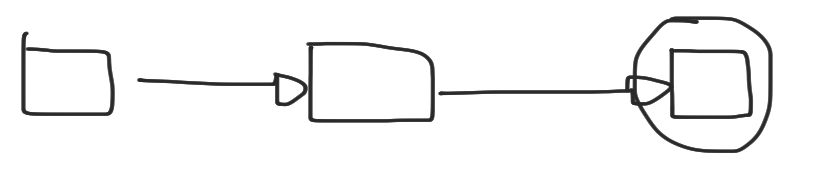
\includegraphics[scale=0.1]{content/graphics/game2}
(we can extend this for any natural number)\\
\textbf{3.} Enforce that the game ends after $\omega$ steps (you cannot bound it from below).
\footnote{
The smallest number of steps required for reachability game to finish is sometimes called the
\textbf{strength of a reachability game}.
}\\
We create such infinite graph:
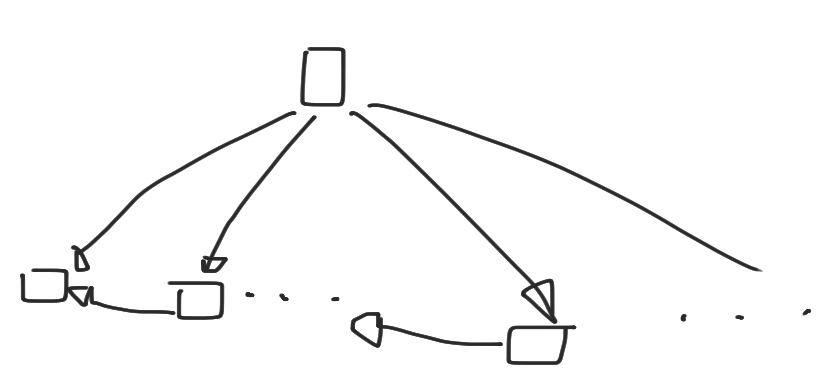
\includegraphics[scale=0.1]{content/graphics/game3}\\
\textbf{4.} Same for $\omega+1$ -- add one more $v_I$ to the previous graph\\
\textbf{5.} $\omega + \omega$ -- copy the graph, the output from first copy goes into the initial vertex of the second one\\

\noindent
$f : V \rightarrow V$\\
$f(S) = S'$, $S \subseteq S'$\\
$S' = \{v \in V\ |\ \forall_{v'} E(v,v') \rightarrow v' \in S\}
\cup \{v \in V\ |\ \exists_{v'} A(v,v') \rightarrow (v,v') \in E\} \cup S$\\
$f^{\alpha}(F) = S_{\alpha}$\\
$S_0 = F$\\
$S_{\alpha} \leftarrow$ set of winning positions of Eve\\
strenght of game = smallest $\alpha$ s.t. $v_I \in f^{\alpha}(F)$\\

\noindent
\textbf{6.} Given a reachability game $G = \langle V, W \rangle$, compute the set $W_E$ ($W_E = \{v\ |\ \text{Eve has a winning strategy from } v\}$).\\
\begin{lstlisting}
S = F;
S' = f(S);
while(S != S') {
 S = S';
 S' = f(S);
}
return S;
\end{lstlisting}

\subsection*{Parity games}
\textbf{Parity condition}:\\
$\{w \in \Gamma^{\omega}\ |\ w = a_0a_1a_2...a_n..., \lim\sup a_n \text{ is even }\}$ where $\Gamma \subseteq \mathbb{N}$\\
\textbf{Theorem}: Parity games are positionally determined.\\

\noindent
\textbf{7.} Let $G$ be a parity game, i.e. $G = \langle B, \textsc{Parity} \rangle$,
s.t. $V_A = \emptyset$ (only Eve moves). Compute the set of winning positions for Eve.\footnote{Since we are looking for an algorithm, assume graph $G$ is finite in size.}\\
\underline{Observation} $v \in V$ is a winning position iff we can reach from $v$ a loop $x_0...x_n$ s.t. the highest priority in the loop is even.
\underline{Proof}
\begin{itemize}
	\item[$\Leftarrow$] easy
	\item[$\Rightarrow$] $\exists \rightarrow$ $(v=v_1)v_2v_3...v_n...$ with ranks $a_1a_2a_3...a_n... \rightarrow$ winning. The highest priority occurring
	infinitely often is even, let's call it $a$.\\
	Thus $\underset{n_0}{\exists:} \underset{n \geq n_0}{\forall} a_n \leq a$\\
	Take a sequence $a_{n \geq n_0}...a...a....a....a$. So we choose a path between two occurrences of $a$ and loop it.
\end{itemize}
\textbf{HOME} Describe the algorithm basing on the observation.
